\chapter{Theory}\label{cha:intro}

\section{Machine learning}\label{sec:research:history}
Machine learning has a wide range of applications. It has proven especially useful for image classification and detection. While neural networks has a long history, applying them to detection problems is a more recent development. This is due to an increase in available computing power.
\subsection{Neural Networks}\label{sec:research:history}

\subsection{Convolutional Neural Networks}
In recent years, a kind of neural network has proven to be especially effective at image and video recognition, i.e. Convolutional Neural Networks (CNN). Instead of manually choosing which features to focus on when training a neural network, the CNN algorithm can take a whole image as input and dimensionally reduces this data in order to decrease the number of computations needed. This is done by convolving the image with trainable convolution kernels. The upside to this is that no potentially useful information must be removed when manually pre-processing the image.
Convolutional neural networks are inspired by the organization of the animal visual cortex, and are variations of multilayered neural networks.

\subsection{Max pooling}
Max pooling is a method used to decrease computational cost and prevent over-fitting a network. The aim is to downsample an input by applying a max filter to sub-regions of the original representation. Figure \ref{fig:maxpooling} gives a simple example of how this is done.

\begin{figure}[h!]
    \centering
    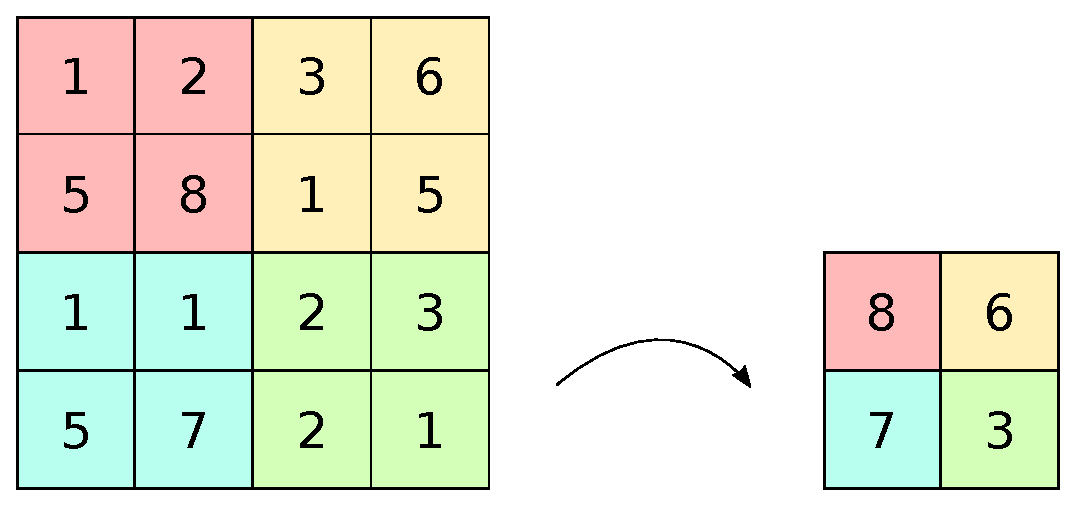
\includegraphics[width=\textwidth]{maxpooling}
    \caption{Simple example showing how max pooling works, with a stride of 2.}
    \label{fig:maxpooling}
\end{figure}

\subsection{Dropout}
Dropout is a technique that reduces over-fitting. At each training stage, or epoch, individual nodes are either removed, i.e. "dropped out" with a probability $1-p$ or kept with a probability $p$. This is essentially the same as using $2^n$ neural networks and combining their outputs, where $n$ is the number of training epochs. 

\section{Problem outline}
